%!TEX root = main.tex
\section{Data and User Models\label{sec:datamodel}}

In this section, we first describe our data model by reporting our data, visualization and query setup, and the underlying lattice of data subsets. We then discuss how analysts explore the lattice through a formative user study, and introduce our user model based on the findings of this study. Finally, we present our problem of finding an informative-and-interesting set of visualizations from the lattice.

\subsection{Structure of visualization stories\label{sec:structure}}
%While the user model used in \system aligns with these findings, our work is the first to present a system that recommends a connected visualization sequence in a hierarchical layout summarizing the space of data subsets.

% \subsection{Data Model}
% We start by discussing the data, visualization and query setup.

% \textbf{Data.}
%\npar \stitle{Data:} We assume that we are operating on a dataset consisting of a single relational table $R$ with dimensions and measure attributes. Our approach also generalizes to multiple tables obeying a star or a snowflake schema \cite{levene2003snowflake}, but we focus on the single table case for ease of presentation.

%\textbf{Visualization.} We define the notion of a visualization for our problem. There are different visualization types such as bar charts, scatter plots, and trend lines, but across all types, a visualization can be defined using five main components: (i) the x-axis attribute(s), (ii) the y-axis attribute, (iii) the subset of data used, (iv) the binning and aggregation functions for the x- and y- axes, and (v) the type of visualization (e.g., bar chart, scatter plot).

%\textbf{Visualization.} We define the notion of a visualization for our problem. In our setup, a visualization can be defined using five main components: (i) the x-axis attributes, (ii) the y-axis attribute, (iii) the subset of data used, (iv) the aggregation function for the y- axis, and (v) visualization type, e.g., bar chart. For example, the Election Polls dataset (used for Figure 1) has four attributes: {\tt Id} (random id for each voter), {\tt Gender} (of the voter), {\tt Race} (of the voter), and {\tt Candidate} (who the voter elected); and the first visualization in Figure 1 can be defined using these attributes as: (i) {\tt Candidate}, (ii) {\tt Id}, (iii) {\tt Gender = Male}, (iv) {\tt Percentage}, (v) {\tt Bar}. We can similarly define other visualizations from this dataset. Note that, even for the same x- and y- axis attribute, aggregation function (for y- axis), and chart type (say Bar), we have a different visualization for each data subset. In Figure 1, we present all except one (the overall) bar charts that show the distribution of vote (corresponding to {\tt Percentage} of {\tt Id}) for 2016 US election candidates (values of {\tt Candidate}), for different demographic groups (the combination of {\tt Gender} and {\tt Race}).
\npar \stitle{Data Model:} We consider the common visual analytics scenario where a dataset consists of a relational table $R$ with \textit{dimensions} attributes to be filtered upon and \textit{measure} attributes to be aggregated upon. A visualization of this dataset consist of: (i) {\tt X}: x-axis attributes, (ii) {\tt Y}: y-axis attribute, (iii) {\tt C(Z)}: filter constraints that specify the data subset, (iv) {\tt A}: aggregation functions for the x- and y- axes. For example, the aforementioned elections dataset has four attributes: voter's {\tt ID}, voter's {\tt Gender}, voter's {\tt Race}, and the {\tt Candidate} that the voter voted for. As shown in Figure \ref{fig:elections_example}, even for the same x- and y- axis attribute, aggregation, and chart type, there can be different visualizations corresponding to different demographic groups (the combination of {\tt Gender} and {\tt Race}). Such visualizations can be written as \textsc{SQL} query: {\tt SELECT X, A(Y) FROM R WHERE C(Z) GROUP BY X}.\footnote{Note that our method directly applies to all counting-based aggregation functions on {\tt Y}, such as \textsc{COUNT}, \textsc{SUM}, \textsc{AVERAGE}, \textsc{PERCENTAGE}. However, our method is not directly applicable to other aggregate functions, such as \textsc{MIN}, \textsc{MAX}, \textsc{MEDIAN}.}
% \dor{possibly ignore discussion of visualization type and just say we focus on bar chart since its most common and cite.} , and (v) visualization type (e.g., bar chart, scatter plot)
\npar Given a set of visualizations $V$ with the same $X$ and $Y$ and different $C(Z)$, we extend the set-theory based \emph{containment} relationships for data subsets and organize the visualizations into a \textit{lattice} as depicted in OLAP data cube literature~\cite{Xin2007}. A visualization $V_i$ (defined by filters $C_a$) is a \textit{parent} of the visualization $V_i^j$ (defined by filters $C_b$) if $C_b$ can be obtained from $C_a$ by adding one additional filter constraint. For example in Figure~\ref{fig:elections_example}, the visualizations (b) Female and (d) Black are the parents of the (h) Black Female visualization. Based on the containment relationship of visualizations, we can organize the visualizations from $V$ to form a lattice, as exemplified in Figure~\ref{fig:lattice}. The lattice contains all visualizations with same x- and y- axes for different data subsets, arranged based on the parent-child relationships between visualizations. The choice of a filter-based data lattice is supported by research in visualization storytelling showing that people prefer visualization sequences structured hierarchically with increasing levels of aggregation~\cite{Kim2017,Hullman2017,Hullman2013}. Given this structure describing the space of possible visualizations, we will now discuss how the edge utility of visualizations in this lattice is defined.
% \textbf{Containment.} Given a data subset defined by a set of constraints $C = \{Z_1 = z_1, \ldots, Z_n = z_n\}$, expanding $C$ by adding one or more new constraints will generate a new data subset that is contained within the former subset. An ancestor-descendant relationship exists between these data subsets. Specifically, a data subset defined by constraints $C_a$ is an ancestor of a data subset defined by constraints $C_b$, if and only if $C_b \subsetneqq C_a$. Further, a data subset defined by constraints $C_a$ is a parent of a data subset defined by constraints $C_b$, if and only if $C_b \subsetneqq C_a \land \mid C_a \mid - \mid C_b \mid = 1$. For example, given a dataset with three attributes {\tt \{P, Q, R\}}, the data subset defined by constraints {\tt \{P = 0,Q = 1\}} has two parents--- the data subset defined by constraint {\tt \{P = 0\}} and the data subset defined by constraint {\tt \{Q = 1\}}.
% \textbf{Lattice.} Based on the containment relationship, we can organize the data subsets of a given dataset to form a hierarchy. This hierarchy of data subsets is overlaid on top of the lattice of attribute combinations. For the rest of the paper, we refer to this data subset hierarchy (overlaid on top of attribute lattice) as \emph{lattice}. In Figure~\ref{fig:lattice} we show the lattice of data subsets for a dataset with three attributes {\tt \{P, Q, R\}}, where we highlight the data subsets that belong to the same attribute combination with the same color. For example, all data subsets with three filters (at the lowest level of hierarchy) belong to the same attribute combination {\tt \{P, Q, R\}}, and are highlighted in gray.

\begin{figure*}[ht!]
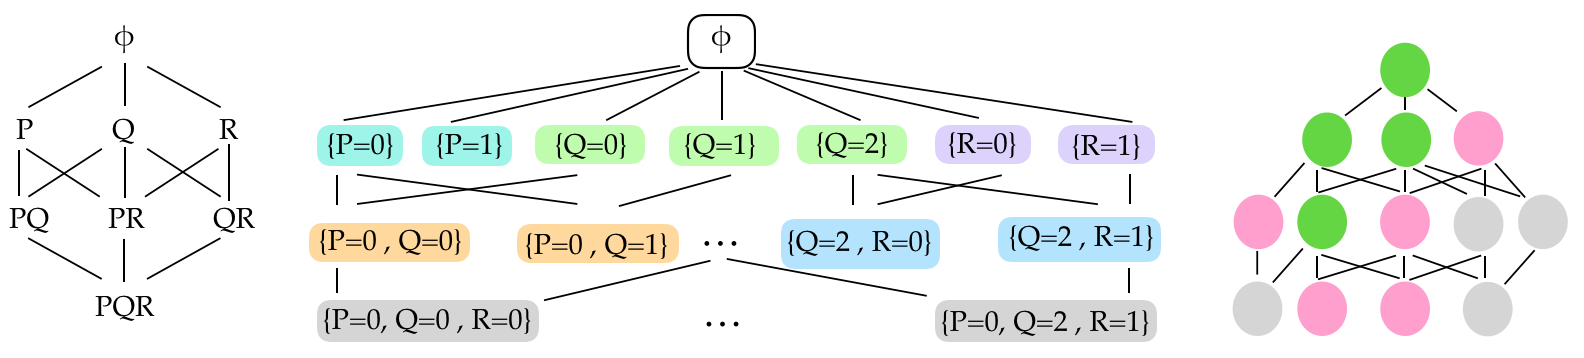
\includegraphics[width=\linewidth]{figures/lattice_frontier.png}
\caption{Left, Middle: Example data subset lattice for a dataset with three binary attributes {\tt \{P, Q, R\}}. The data subsets that belong to the same attribute combinations are highlighted with same color. $\phi$ represents the overall distribution (where no filter conditions is applied). Right: Toy example demonstrating the notion of ``frontier''. Green nodes are selected in the dashboard. The neighbors of the set of selected green nodes are the frontier nodes, shown in pink. Other unpicked nodes in the lattice are shown in gray.}
\label{fig:lattice}
\end{figure*}
%We now extend the concept of \emph{containment} for visualizations defined according to our setup.

% \textbf{Viz Containment.} Let $V$ be the set of visualizations (of same type) that show the same $X$ and $Y$ for different $C(Z)$. Given a visualization $V_i \in V$, a parent of $V_i$, $V_i^j$ ($V_i^j\in V$) is a visualization that corresponds to a parent data subset of the former. In Figure~\ref{fig:elections_example} we present three visualizations that show the distribution of votes for 2016 US election candidates in three demographic groups: (i) female voters, (ii) black voters, (iii) black female voters. As per the parent-child relationship among the data subsets, the visualizations corresponding to (i) and (ii) are parents of the visualization corresponding to (iii).

% \begin{figure}[bht]
% \centering
% 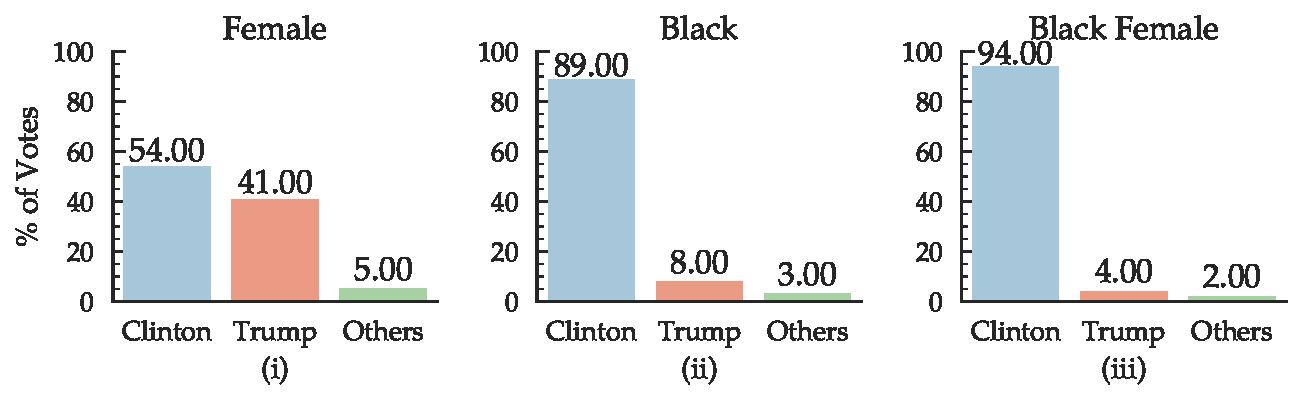
\includegraphics[scale=0.4]{figures/US_Election_Parent_Child.pdf}
% \caption{Parent-child relationship amongst visualizations that show the distribution of votes for 2016 US election candidates in three demographic groups: (i) female voters, (ii) black voters, (iii) black female voters.}
% \label{fig:elections_example}
% \end{figure}

%\haz{Perhaps it will look better if have (iii) in a new line (and centered) to quickly reflect the parent-child relationship.}\dor{Considering that this will take up more space also not sure whether not sure we should mix up the problem formulation with the model itself. Himel?}

% \textbf{Viz Lattice.} Based on the containment relationship of visualizations, we can organize the visualizations from $V$ to form a lattice. This lattice contains all visualizations (of same type, e.g., bar charts) that show the same x- and y- axes for different data subsets, and arranges them as per the parent-child relationships between data subsets. Our goal is to traverse this lattice of visualizations, and identify informative and interesting visualizations.

\subsection{Utility of Visualizations: User Expectation Model\label{sec:utility}}
In order to identify which visualizations should be picked from the lattice, we first conduct a formative user study
to study how the presence of one or more observed parents in the visualization lattice affects an analyst's perception of an unseen visualization. Using these findings, we then model the effective utility of displaying an unseen visualization to a user in the context of seen visualizations.% by defining metrics of \textit{interestingness} and \textit{informativeness}.
%to study how analysts interpret parent-child relationships in a visualizations lattice, and then model the effective utility of displaying an unseen visualization to a user in the context of seen visualizations.
%\textbf{Top Down Traversal.} We observe that, while exploring a dataset, users first look at the top level visualizations before looking at the next level \cite{Kim2017, Hullman2013}. Further, the data distributions learnt from the top level visualizations induce user expectation for the next level. For example, in Example 1, a journalist is likely to examine the voting trends of female or black voters before examining the voting trends of black female voters, and his/her expectation of black female voters would be affected by the observed reference(s) (female or black voters). Based on these two observations, we model user expectation $\hat{V_i}$ corresponding to an unseen visualization $V_i$ based on its seen/observed parents $O(V_i) = \{V_i^1, \ldots, V_i^\lambda\}$ in the visualization lattice.

\stitle{Formative User Study:} %We conducted a user study to understand how a user's perception of an unseen visualization is affected by one or more of its observed parents.
We recruited 9 participants in a study to predict the distribution of an unseen visualization with two constraints. Participants were asked to make a prediction regarding an unseen visualization after seeing the first parent displayed and subsequently after seeing the second parent displayed. For the chosen visualization parents, the first parent have data distributions that very closely follows that of the unseen visualization, whereas the second parent differs greatly from the unseen visualization. In this between-group study, one group of participants (G1) were shown the first parent followed by the second parent, whereas another group of participants (G2) were shown the second parent followed by the first parent. We examined how users form their expectation in presence of these observed parents. The results are summarized in Figure \ref{fig:formative_study}. Our main findings are: (1) participants naturally form their expectations based on one or more observed parents; (2) seeing a parent that well describes the unseen visualization leads participants to better estimate the unseen visualization; (3) in absence of an informative parent, participants can be misled to form an inaccurate expectation; (4) in presence of  both informative and uninformative parents, the variance of expectation increases compared to just seeing the informative parent.
\begin{figure}[h!]
\centering
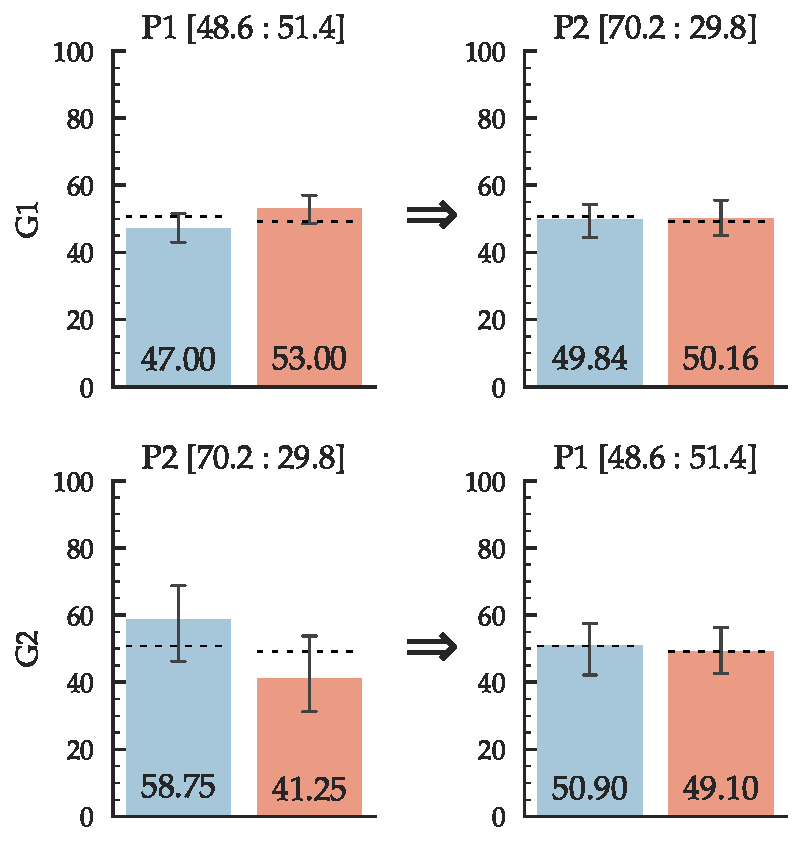
\includegraphics[width=\linewidth]{figures/Formative_Study.pdf}
\caption{Bar charts and error bars showing the mean and variance of participants' estimated distribution during the formative user study. Group 1 (G1) participants were shown the informative parent first, followed by the uninformative parent; whereas Group 2 (G2) participants were shown the uninformative parent first, followed by the informative parent. G1 participants closely approximated the unseen visualization immediately after seeing the informative parent. The ground truth values for the unseen visualizations are shown as dotted lines and printed in square brackets in the visualization title.}
\label{fig:formative_study}
\end{figure}
\npar Based on these findings, we model two aspects of the unseen-visualization and observed-parent relationship through its \textit{interestingness} and \textit{informativeness} criteria.
\stitle{Informativeness:} To model the informativeness of an observed parent in the context of an unseen visualization, we characterize the capability of the parent in predicting the unseen visualization. As highlighted in finding (2), an observed parent is \emph{informative} if its data distribution closely follows the data distribution of the unseen child visualization, since the visualization helps the analyst form an accurate mental picture of what to expect from the unseen visualization. Specifically, we formulate the informativeness of an observed parent $V_i^j$ of an unseen visualization $V_i$ as the similarity between their data distributions measured using a distance function $D(V_i, V_i^j)$. The most informative parents $V_i^*$ of an unseen visualization $V_i$ are the ones whose data distributions are most similar to the unseen.
\begin{equation}
    V_i^*=\underset{V_i^j}{argmin}\ D(V_i, V_i^j)
\end{equation}
Since our finding (4) demonstrates how seeing multiple parents can lead to worser visualization understanding, we allow users to specify a threshold $\theta$ to control the degree of similarity for which a parent can be declared as an informative, such that the distance $D(V_i, V_i^{*, \theta})$ corresponding to the informative parents $V_i^{*, \theta}$ are at least $\theta\%$ close to its most informative parent:
\begin{equation}
    V_i^{*, \theta} = \{V_i^j : \frac{D(V_i, V_i^*)}{D(V_i, V_i^j)} \geq \theta\}
\end{equation}
%Since declaring a parent as informative can vary depending on its similarity with the unseen compared to other parents, we allow the user to specify a threshold $\theta$, which we expect to be close to 1.0, such that the similarity score $S(V_i, V_i^{*, \theta})$ corresponding to the informative parents $V_i^{*, \theta}$ are at least $\theta\%$ of that of the most informative parents'.
For example, if $\theta = 0.8$, all parents of $V_i$ whose similarity scores are at least 80\% compared to $V_i^*$ are deemed as \textit{informative}. In Figure~\ref{fig:elections_example}, while both visualization (b) and (d) are considered parents of visualization (h), only visualization (d) (Black) are considered the informative parent of visualization (h) (black female population), for any values of $\theta \geq 11\%$ via the Euclidean distance metric. Note that, our proposed system can work with different distance metrics such as cosine similarity and earth mover's distance. Without loss of generality, we chose to use Euclidean distance metric for the remainder of our paper.

%the visualization corresponding to black voters is the most informative parent of the visualization corresponding to black female voters. For $\theta <= 0.11$, the former remains the only informative parent of the latter.

\stitle{Interestingness:} While informative parents contribute to the prediction of an unseen visualization, the most interesting visualizations to recommend are those for which \emph{even the informative parents fail to accurately predict the visualization}. \dor{Can we justify this based on our findings?} To model the interestingness of an unseen visualization $V_i$ in the context of an observed parent $V_i^j$, we characterize the deviation between their data distributions using a distance function $D(V_i, V_i^j)$. The unseen visualizations whose data distributions deviate from the observed informative parents are \emph{interesting}. \cut{The most interesting unseen visualizations $V_\#$ are the ones that deviate most from their observed informative parents.
\begin{equation}
    V_\#=\underset{V_i}{argmax} \ D(V_i, V_i^{*, \theta})
\end{equation}
In Figure \ref{fig:elections_example}, the most interesting visualization to recommend is the one corresponding to white female voters. This visualization significantly differs from its informative parent---the visualization corresponding to female voters.} \dor{The argmax notation not necessary since we're just using this in our utility function. The election example is not convincing, the informative parent of white female is actually white and not female. Also the differences are not too significant.}

%\noindent Additional model extensions can be added to this objective function based user specification. For example, there may be $k$ visualizations that approximately yield equal contribution to the user's expectation. For simplicity of notation, we have assumed $k=1$ in the aforementioned model. In order, a user may want to prevent the recommendation of spuriously interesting subsets of the data. We can discard visualizations that falls below a certain subpopulation size threshold.
\stitle{Subpopulation size consideration:} The danger of spurious patterns and correlations in visualizations that contain small subpopulation size is a well-known problem in exploratory analysis~\cite{Binnig2017}. We take two preventive measures to avoid including such misleading visualization in our dashboards. First, in the lattice generation process discussed in Section~\ref{sec:algorithms}, we allow users to select an `iceberg condition' \footnote{The terminology is used in the discussion of iceberg cubes in OLAP literature~\cite{Xin2007}.} ($\delta$) to adjust the extent of pruning on visualizations whose sizes fall below a certain percentage of the overall population size. Second, we downweigh the interestingness edge utility $U(V_i, V_i^j)$ between a parent $V_i^j$ and a child visualization $V_i$ by the ratio of their sizes:
\begin{equation}
    U(V_i, V_i^j) = \frac{|V_i|}{|V_i^{j}|} \cdot D(V_i, V_i^j)
    \label{edge_utility}
\end{equation}
\subsection{Problem Formulation}
Given the lattice data model and the user model for visualization utility described above, the goal of our system is to generate a dashboard by selecting $k$ visualizations from the lattice. We enforce that the generated dashboard satisfies several requirements:
 \begin{enumerate}
 	\item Dashboard must include the overall visualization (topmost visualization with no filter applied) to serve as reference to the rest of the visualizations in the dashboard.
 	\item For each visualization except for the overall, at least one of its informative parents is included within the $k$ visualizations. This excludes the uninformative parents as exemplified in black female example in the dashboard, especially since our findings 3 and 4 show that showing multiple, improper parents can mislead the participants, resulting in a higher variance across their estimations. %This enforces that every visualization shown in the dashboard has an informative reference to compare against to create a connected story.
 	\item The selected $k$ visualizations are collectively most ``interesting'' in presence of their informative parents as measured by the utility in Equation \ref{edge_utility}.
\end{enumerate}
 The problem of finding a connected subgraph in the lattice that has the maximum combined edge utility is  known as the maximum-weight connected subgraph problem~\cite{ErnstAlthaus2009} and is known to be NP-Complete, via a reduction from the \textsc{Clique Problem}~\cite{Parameswaran2010}. In Section~\ref{sec:algorithms}, we discuss heuristic algorithms used for deriving a locally optimal solution for ensuring interactive runtime.
